%!TEX root = ../thesis.tex

\section{Checking}
\label{sec:checking}

In this section we will outline the process of the actual \textit{verification} of the now implemented architecture.
The verification process itself is threefold:
Before any verification can be done, it needs to be clear what shall be verified - not in the sense what the object of verification is but what its goal is, i.e. which properties express the security of the architecture adequately?
This allows the actual verification of these properties as the next step which will lead to first results.
In the case of a real world verification attempt these results hopefully are that the system to be verified is perfectly valid - it is, however, most likely that at least some of the properties verified will end up with a negative result.
In this case, the model and/or properties are refined which marks the last step.

Not only will we detail these steps themselves, we will also reflect whether this process of verification is trustworthy by shedding light on the methodology of deriving the concretization of these by now only loosely described steps.
To outline this, we will answer two questions:
How do we phrase properties to verify?
How do we refine the model and/or properties on a verification failure?

\subsection{Verification Process}

\subsubsection{Properties}
\label{sec:props}

% TODO: Explain syntax and assumptions of \gls{ltl} properties

In the summary of section \ref{sec:ifc-model} we mentioned that there are some arguments to the information flow semantic functions in $ \I $ that are not used to determine the information flow label of some architectural word.
These induce the first properties we will verify the MINRV8 architecture against.

Firstly, recall the definition of the LOAD and STORE semantics.
The new tracking labels resulting from executing such an instruction solely depend on the labels of the word loaded or stored.
What hasn't been used in the definition of information flow is the label of the target address of the memory operation.
It is intuitive that the address does not influence the label of the information itself.
% TODO: is security a good word?
However, this suggests that the labels of the address of the memory operation might be relevant for the security of architecture as a whole in another.
This leads to the following property:
\begin{enumerate}[label=\Roman*.,series=]
    \item \label{itm:prop-mem-i}
    Whenever a memory operation is performed in privileged mode, the target address must be integrous.

    \begin{lstlisting}[
        language=smv,
        caption={Implementation of property \ref{itm:prop-mem-i}},
        label={snpt:prop-mem-i}
    ]
        LTLSPEC NAME MEMORY_OP_INTEGRITY :=
            assumptions -> G (
                priv & op in { LOAD, STORE }
                -> (regs_integrity[rs1] & 0h_03) = 0h_03
            );
    \end{lstlisting}
\end{enumerate}

% TODO: give intuition for both properties

Secondly, recall the definition of the semantics for \rv{Csrrs} or \rv{Csrrc}, respectively.
These only propagate information flow tracking labels by assigning the constant labels of the \gls{csr} read to the respectively targeted register.
We decided to model the labels of \glspl{csr} as constants because they control the state of the architecture and as such might be target of an attack.
We labelled all \glspl{csr} as integrous and \gls{mstatus} as confidential.
We decided to not label \gls{pmacfg} or \gls{pmpcfg} as confidential since it can be assumed that user mode must be able to know where memory regions are to operate correctly.
% TODO: Phrase this better
Our architecture does not support virtual addresses, address translation or other similar concepts which might hide details of the memory settings from user mode leaving it without the need to know the details of memory settings.

Coming back to the information flow semantics of \rv{Csrrs} and \rv{Csrrc}, notice that in the respective definition of the semantical functions the value the \glspl{csr} are written with is not used.
This must necessarily be the case since the labels of the \glspl{csr} are constant and as such can not change based on the labels of the value to write them with.
However, this leads us to phrase a property about the \gls{csr} labels that ensures their integrity:
\begin{enumerate}[label=\Roman*.,resume]
    \item \label{itm:prop-csr-i}
    Whenever a \gls{csr} is written, the value it is written with must be integrous.

    \begin{lstlisting}[
        language=smv,
        caption={Implementation of property \ref{itm:prop-csr-i}}
    ]
        LTLSPEC NAME CSR_INTEGRITY :=
            assumptions -> G (
                priv & op in { CSRRS, CSRRC }
                -> regs_integrity[rs2] = 0h_FF
            );
    \end{lstlisting}
\end{enumerate}

From all the variables our implementation of the MINRV8 architecture comprises we now considered \smv{regs} and \smv{memory} as well as \smv{cache} in regards to the security of the architecture by looking at the gaps of the information flow semantic functions.
We also considered the variable \smv{csrs} by assigning constant information flow labels to it and using it as an information flow target, i.e. we phrased properties ensuring that certain flows of information \textit{to} \smv{csrs} do not occur.
However, up to this point we only implicitly handled the \smv{priv} variable which holds the current privilege mode.
It was used as a source of labels since it determines the labels of machine words loaded as immediates by LOADI.

It is reasonable to assume, though, that \smv{priv} also can serve as an information flow target; similar to \smv{csrs}.
We already did this partially for property \ref{itm:prop-mem-i} where we assumed the architecture to be in privileged mode.
These properties, however, only dealt with the integrity labels of information.
The domain of confidentiality has yet been left out so we will introduce one final property for verification that covers the interplay between privilege mode and confidentiality labels:
\begin{enumerate}[label=\Roman*.,resume]
    \item \label{itm:prop-no-leak}
    Whenever the architecture is in user mode, there is no confidential data in any register.

    \begin{lstlisting}[
        language=smv,
        caption={Implementation of property \ref{itm:prop-no-leak}},
        label={snpt:prop-no-leak}
    ]
        LTLSPEC NAME NO_LEAK :=
            assumptions -> G (priv | (
                regs_conf[0] = 0h_00
                & regs_conf[1] = 0h_00
                & regs_conf[2] = 0h_00
                & regs_conf[3] = 0h_00
            ));
    \end{lstlisting}
\end{enumerate}

% TODO: reflect removed properties MSTATUS_CONFIDENTIAL and MEMORY_OP_CONFIDENTIAL; why is it not sensible to control public input?

\subsubsection{Mitigations \& Refinement}

% TODO: Make sure this is mentioned in the introduction
% TODO: Reflect goal of the thesis once it has been set up properly in the introduction
With these properties at hand we can introduce our approach to the verification-refinement loop that has been mentioned initially in section \ref{sec:introduction} as well as the introduction of this section and which is depicted in figure \ref{fig:ver-process}.
Formal verification does not end when a verification procedure returns some result.
If such a result happens to be a negative one, a formal verification researcher must be able to answer to questions:
\begin{enumerate}
    \item \label{itm:counter-ex-validity}
    Is the negative result legitimate?
    \item \label{itm:counter-ex-mitigation}
    If so, how can the uncovered vulnerability to the system be mitigated?
\end{enumerate}

In this thesis, the result of a failed attempt to verify the MINRV8 architecture against some property will be a counter-example trace including an initial state and a sequence of instructions finally leading to the violation of the given property.
% TODO: Argue for why it is not sensible to verify our implementation of the specification
To answer question \ref{itm:counter-ex-validity}, we simply must inspect the trace at hand and verify whether all state transitions and variable changes are indeed valid in regard to the specification of MINRV8.
If the answer to this question is no, the implementation has to be fixed accordingly and the proofs must be re-run.

If, however, it is found that the counter-example produced by nuXmv is genuine, it must be decided how the newly found vulnerability is handled.
As already mentioned in the introduction, there are two ways to handle a vulnerability.
Either it is a proper architectural vulnerability that must be mitigated accordingly by architectural measures or it simply sheds light on a vulnerable \textit{usage} of the architecture that cannot be mitigated appropriately without removing critical features from the architecture itself.
For example, an obvious counter-example for property \ref{itm:prop-no-leak}, that no information can leak to user mode, would be that machine-mode simply hands confidential data to user mode.
No sensible architectural mechanisms could prevent machine mode from doing this as long as machine mode is in fact able to hand data to user mode - which it should be.

In the first case, where we discover a counter-example to comprise a proper architectural vulnerability, we will try to find mechanisms that mitigate the respective vulnerability and also attempt to verify the effectiveness of such mitigations by re-running the proofs.
If however, we do not find the counter-example to use a vulnerability but rather to describe \textit{vulnerable code}, we will phrase rules for programmers that prohibit such bad code patterns and add these rules to the global assumptions for the properties.
We also will then verify the effectiveness of these rules by re-running the proofs again.

\begin{figure}
    \centering
    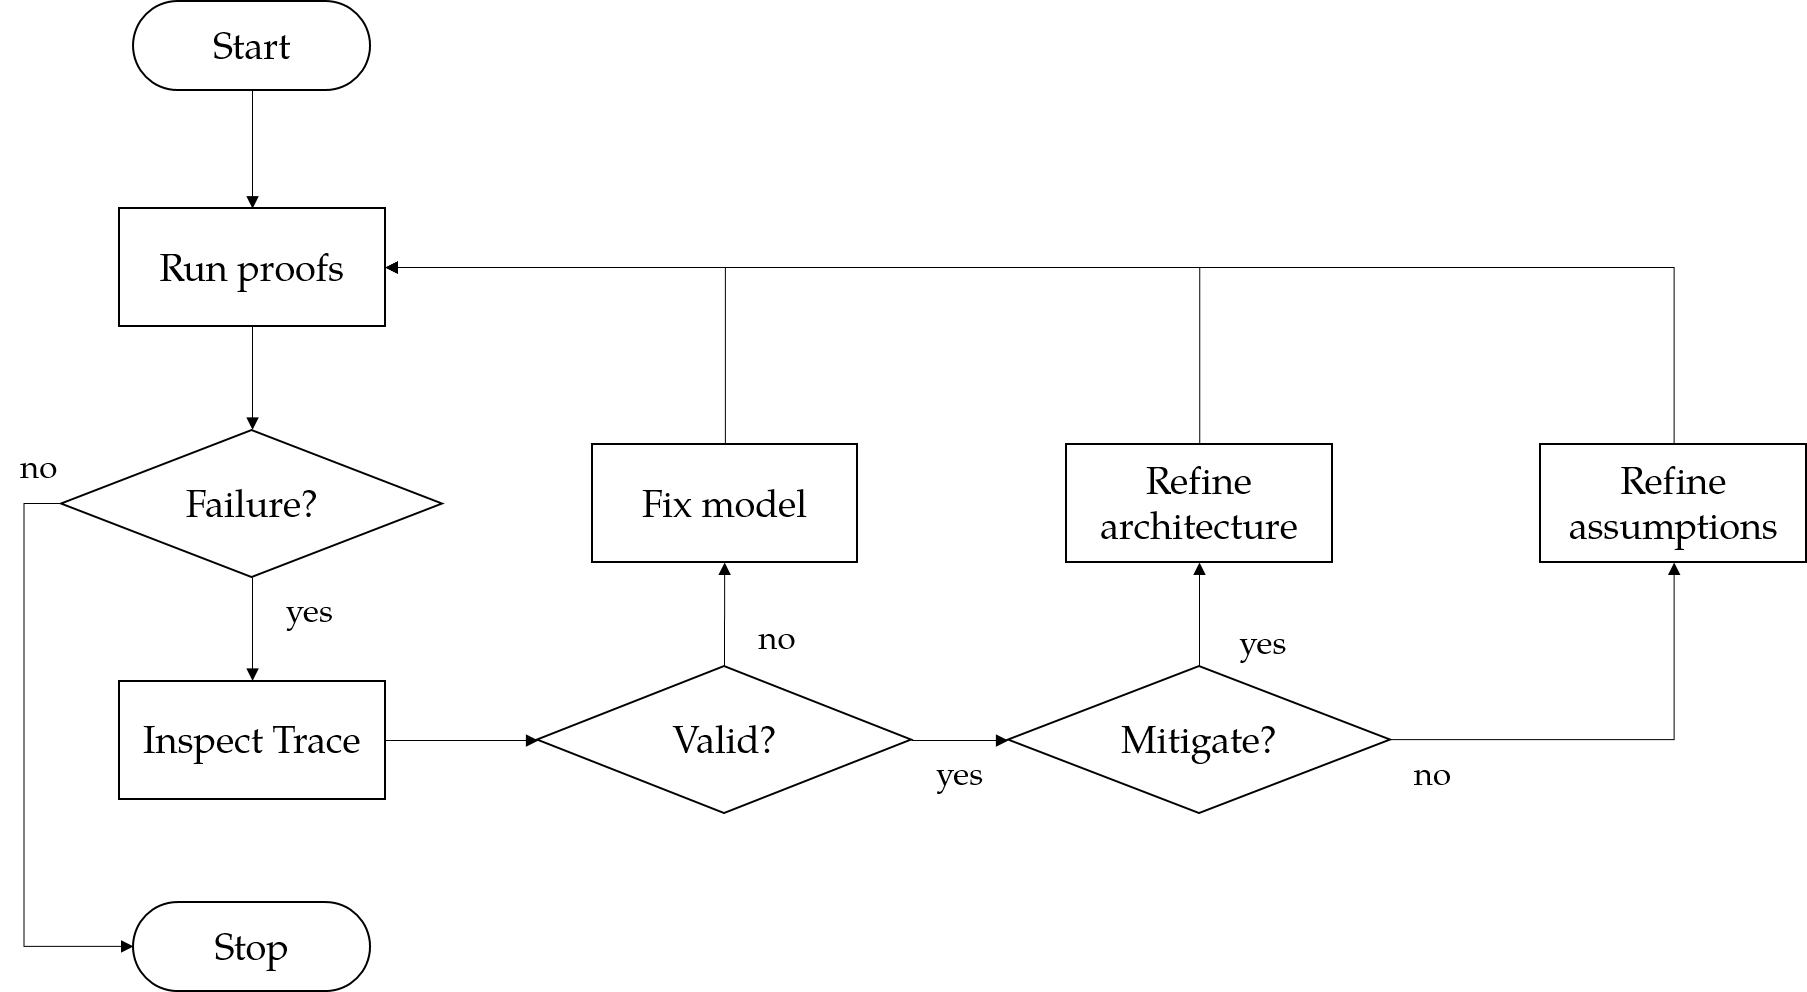
\includegraphics[width=\textwidth]{figures/verfification-process.png}
    \caption{Verification Process Flowchart}
    \label{fig:ver-process}
\end{figure}

% TODO: Use graphic
\begin{figure}
    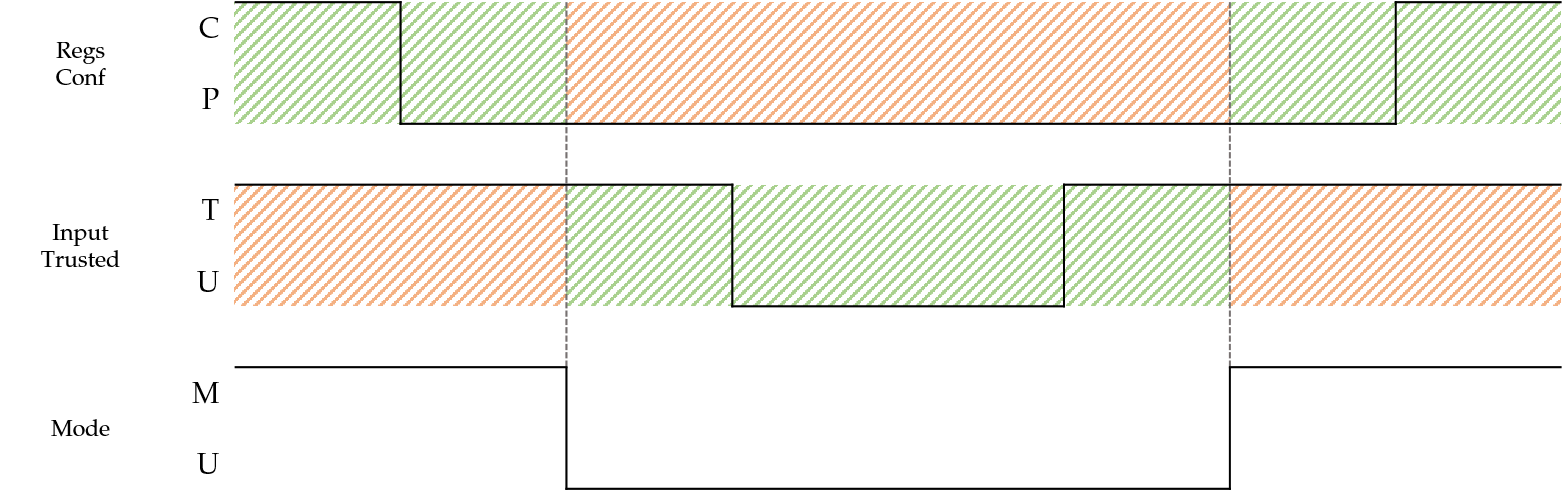
\includegraphics[width=\textwidth]{figures/properties.png}
\end{figure}
